\documentclass[xetex,mathserif,serif]{beamer}
\usepackage{polyglossia}
\setdefaultlanguage[babelshorthands=true]{russian}
\usepackage{minted}
\usepackage{tabu}
\usepackage{moresize}

\useoutertheme{infolines}

\usepackage{fontspec}
\setmainfont{FreeSans}
\newfontfamily{\russianfonttt}{FreeSans}

\definecolor{links}{HTML}{2A1B81}
\hypersetup{colorlinks,linkcolor=,urlcolor=links}

\setbeamertemplate{blocks}[rounded][shadow=false]

\setbeamercolor*{block title alerted}{fg=red!50!black,bg=red!20}
\setbeamercolor*{block body alerted}{fg=black,bg=red!10}

\tabulinesep=1.2mm

\title{Веб-программирование}
\author[Юрий Литвинов]{Юрий Литвинов\\\small{\textcolor{gray}{yurii.litvinov@gmail.com}}}
\date{29.11.2019г}

\newcommand{\attribution}[1] {
\vspace{-5mm}\begin{flushright}\begin{scriptsize}\textcolor{gray}{\textcopyright\, #1}\end{scriptsize}\end{flushright}
}

\begin{document}

	\frame{\titlepage}

	% \section{Доклады}

	% \begin{frame}
	% 	\frametitle{Доклады}
	% 	\begin{itemize}
	% 		\item unsafe, fixed, P/Invoke
	% 		\begin{itemize}
	% 			\item \url{https://docs.microsoft.com/en-us/dotnet/csharp/language-reference/keywords/unsafe}
	% 			\item \url{https://docs.microsoft.com/en-us/dotnet/csharp/programming-guide/unsafe-code-pointers/index}
	% 			\item \url{https://docs.microsoft.com/en-us/dotnet/csharp/language-reference/keywords/fixed-statement}
	% 			\item \url{https://docs.microsoft.com/ru-ru/cpp/dotnet/how-to-call-native-dlls-from-managed-code-using-pinvoke}
	% 		\end{itemize}
	% 		\item Интернирование строк
	% 		\begin{itemize}
	% 			\item \url{https://habr.com/post/224281/}
	% 		\end{itemize}
	% 		\item Rx.NET
	% 		\begin{itemize}
	% 			\item \url{https://habr.com/post/242613/}, \url{http://introtorx.com/}
	% 		\end{itemize}
	% 		\item TPL.Dataflow
	% 		\begin{itemize}
	% 			\item \url{https://docs.microsoft.com/en-us/dotnet/standard/parallel-programming/dataflow-task-parallel-library}
	% 			\item \url{https://habr.com/post/138531/}
	% 		\end{itemize}
	% 	\end{itemize}
	% \end{frame}

	\section{Введение}

	\begin{frame}
		\frametitle{Веб-приложения}
		\framesubtitle{Как оно вообще работает}
		\begin{itemize}
			\item Пользователь заходит браузером на определённый URL
			\begin{itemize}
				\item На самом деле, выполняя HTTP GET-запрос на порт 80 или 443 (обычно)
			\end{itemize}
			\item ОС сервера перенаправляет запрос запущенному там \textit{веб-серверу}
			\begin{itemize}
				\item Например, Apache, IIS
			\end{itemize}
			\item Веб-сервер --- отдельный процесс, в рамках которого запущено несколько \textit{веб-приложений}, веб-сервер по URL запроса определяет, какому веб-приложению он адресован, и передаёт запрос ему
			\item Веб-приложение формирует ответ и отправляет его обратно по HTTP в виде HTML-страницы
			\item Эта страница и показывается пользователю в браузере
		\end{itemize}
	\end{frame}

	\begin{frame}
		\frametitle{Веб-сервисы}
		\begin{itemize}
			\item \textit{Веб-сервис} --- это примерно то же самое, но не для пользователя, а для других приложений
			\item Нужны для создания распределённых приложений
			\item Общаются не с помощью HTML, а посредством специализированных протоколов
			\begin{itemize}
				\item Например, SOAP 
				\begin{itemize}
					\item Использует синтаксис XML, может использовать HTTP как транспорт
				\end{itemize}
			\end{itemize}
			\item Как правило, содержат механизм публикации метаинформации
			\begin{itemize}
				\item Например, WSDL
			\end{itemize}
			\item Реализуются посредством технологий, например, Windows Communication Foundation
		\end{itemize}
	\end{frame}

	\begin{frame}
		\frametitle{Веб-приложения и .NET}
		\begin{itemize}
			\item Веб-сервер --- IIS (Internet Information Services), IIS Express, Kestrel
			\begin{itemize}
				\item Есть ``из коробки'' в Windows, IIS Express поставляется с Visual Studio и используется для отладки
			\end{itemize}
			\item Технология для разработки веб-приложений --- ASP.NET MVC
			\begin{itemize}
				\item ASP.NET MVC 5
				\item ASP.NET MVC Core 3.0
			\end{itemize}
			\item Технология для разработки веб-сервисов --- WCF
			\item Работа с базами данных --- MS SQL Server (SQL Server Express)
			\item ORM --- Entity Framework (Entity Framework Core)
			\item Облачный хостинг --- Azure
		\end{itemize}
	\end{frame}

	\section{Фронтенд}

	\begin{frame}
		\frametitle{Браузерная часть}
		\begin{itemize}
			\item HTML (HyperText Markup Language) --- используется для задания содержимого и структуры веб-страницы
			\begin{itemize}
				\item Тут размечаются параграфы, заголовки, списки, таблицы и т.д.
				\item Тут же обычно определяются способы идентифицировать элементы
			\end{itemize}
			\item CSS (Cascading Style Sheet) --- используется для задания внешнего вида, оформления и расположения элементов
			\item JavaScript --- используется для задания поведения веб-страницы на клиенте
			\begin{itemize}
				\item Интерпретируется браузером
				\item Полноценный язык программирования
			\end{itemize}
		\end{itemize}
	\end{frame}

	\begin{frame}[fragile]
		\frametitle{DOM}
		\begin{itemize}
			\item DOM (Document Object Model) --- представление HTML-документа в виде дерева объектов и API для доступа к нему
			\item JavaScript может манипулировать DOM-деревом, браузер рендерит его ``на лету'', что и даёт интерактивность
		\end{itemize}
		\begin{columns}
			\begin{column}{0.5\textwidth}
				\begin{tiny}
					\begin{minted}{html}
<table class="listing">
    <thead>
        <tr class="odd">
            <th>Выпускник</th>
            <th>Научный руководитель</th>
            <th>Текст</th>
        </tr>
    </thead>
    <tbody>
        <tr class="odd">
            <td>Акбаров Артур Александрович</td>
            <td>д.т.н., проф. Д.В. Кознов</td>
            <td><a href="bmo/441-Akbarov-report.pdf">Текст</a></td>
        </tr>
    </tbody>
</table>
					\end{minted}
				\end{tiny}
			\end{column}
			\begin{column}{0.5\textwidth}
				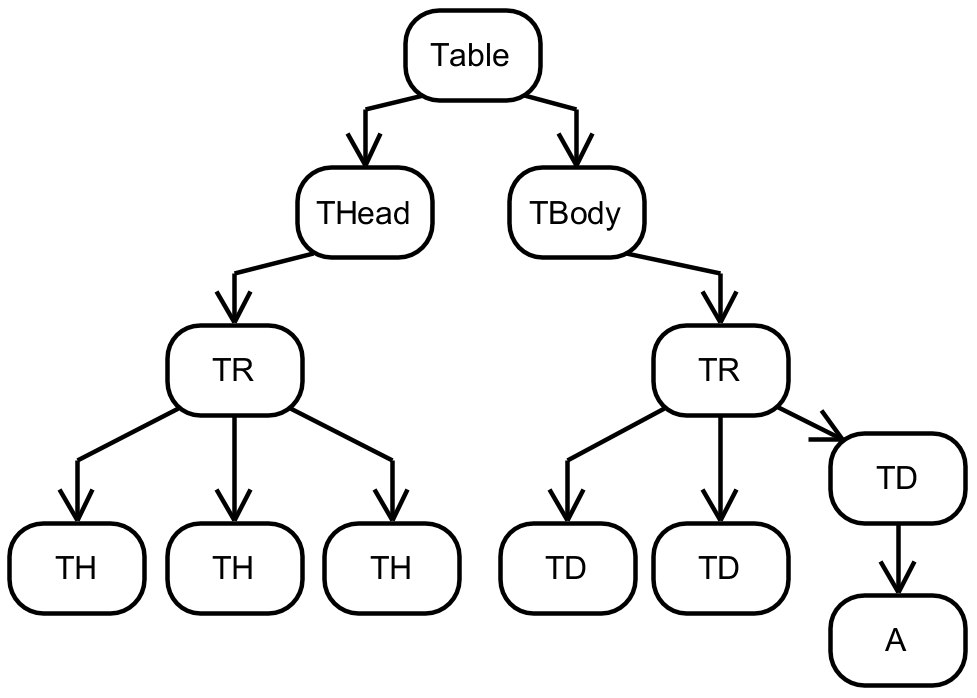
\includegraphics[width=\textwidth]{domTree.png}
			\end{column}
		\end{columns}
	\end{frame}

	\begin{frame}[fragile]
		\frametitle{HTML-формы}
		\begin{itemize}
			\item Способ получить ввод от пользователя
			\item Возможность организовать POST-запрос (GET по умолчанию)
		\end{itemize}
		\begin{minted}{html}
<form method="post">
  First name:<br>
  <input type="text" name="firstName"><br>
  Last name:<br>
  <input type="text" name="lastName"><br><br>
  <input type="radio" name="gender" value="male" checked>Male<br>
  <input type="radio" name="gender" value="female">Female<br>
  <input type="submit" value="Submit">
</form>
		\end{minted}
	\end{frame}

	\begin{frame}[fragile]
		\frametitle{CSS}
		\begin{itemize}
			\item Способ задать внешний вид элементов
		\end{itemize}
		\begin{minted}{html}
<!DOCTYPE html>
<html>
<head>
<style>
  body {background-color: powderblue;}
  h1   {color: blue;}
  p    {color: red;}
</style>
</head>
<body>
<h1>This is a heading</h1>
<p>This is a paragraph.</p>
</body>
</html>
		\end{minted}
		\attribution{https://www.w3schools.com}
	\end{frame}

	\begin{frame}[fragile]
		\frametitle{Или, что более типично}
		\begin{minted}{html}
<!DOCTYPE html>
<html>
<head>
  <link rel="stylesheet" href="styles.css">
</head>
<body>

<h1>This is a heading</h1>
<p>This is a paragraph.</p>

</body>
</html>
		\end{minted}
		\attribution{https://www.w3schools.com}
	\end{frame}

	\begin{frame}[fragile]
		\frametitle{Селекторы}
		\begin{minted}{html}
<p id="p01">I am different</p>
<p class="error">Error message</p>
		\end{minted}
		\vspace{5mm}
		\begin{minted}{css}
#p01 {
    color: blue;
}

p.error {
    color: red;
}
		\end{minted}
		\attribution{https://www.w3schools.com}
	\end{frame}

	\begin{frame}[fragile]
		\frametitle{Немного JavaScript-а}
		\begin{minted}{html}
<!DOCTYPE html>
<html>
<body>

<h1>My First JavaScript</h1>

<button type="button"
onclick="document.getElementById('demo').innerHTML = Date()">
Click me to display Date and Time.</button>

<p id="demo"></p>

</body>
</html> 
		\end{minted}
		\attribution{https://www.w3schools.com}
	\end{frame}

	\begin{frame}[fragile]
		\frametitle{Или так}
		\begin{small}
			\begin{minted}{html}
<!DOCTYPE html>
<html>
<head>
<script>
function doSomething() {
  document.getElementById("demo").style.fontSize = "25px";
  document.getElementById("demo").style.color = "red";
  document.getElementById("demo").style.backgroundColor = "yellow";
}
</script>
</head>
<body>

<button type="button" id="demo" onclick="doSomething()">Click me!</button>

</body>
</html>
			\end{minted}
		\end{small}
		\vspace{-3mm}
		\attribution{https://www.w3schools.com}
	\end{frame}

	\begin{frame}
		\frametitle{AJAX}
		\framesubtitle{Asynchronous JavaScript And XML}
		\begin{center}
			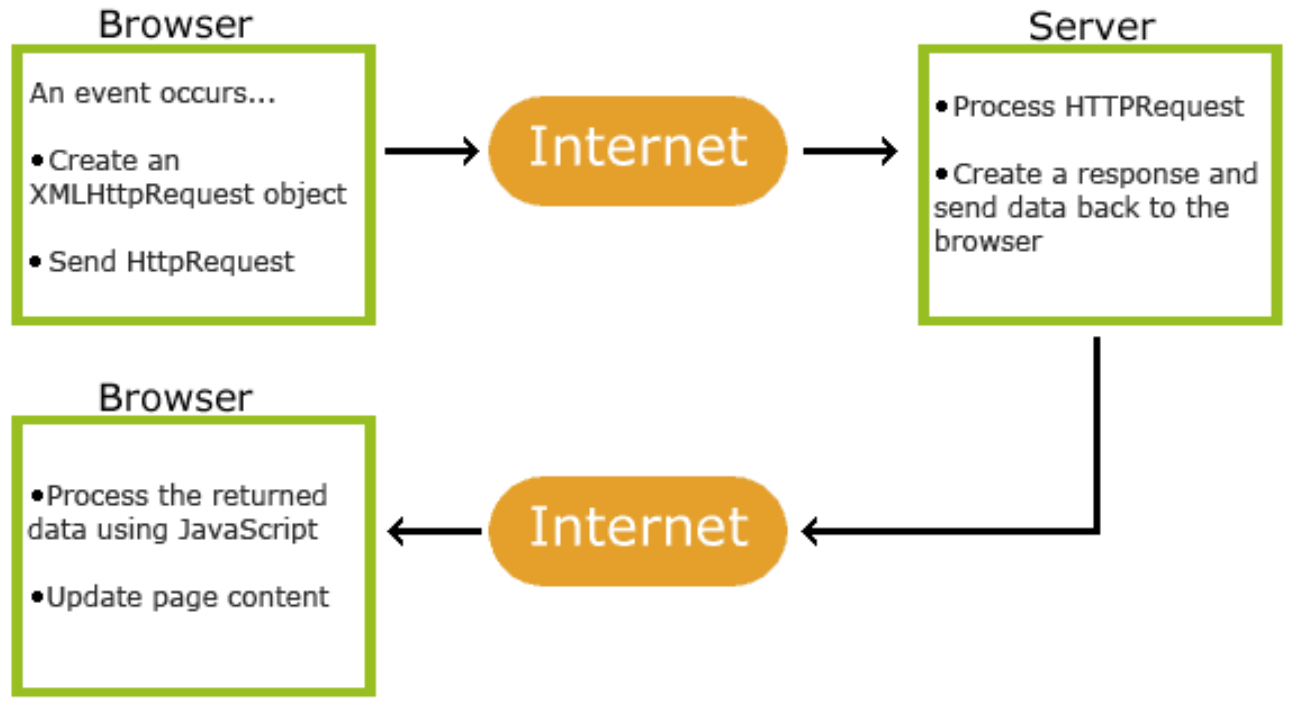
\includegraphics[width=0.7\textwidth]{ajax.png}
		\end{center}
	\end{frame}

	\begin{frame}[fragile]
		\frametitle{Пример}
		\begin{scriptsize}
			\begin{minted}{html}
<!DOCTYPE html>
<html>
<body>
<div id="demo">
  <h2>The XMLHttpRequest Object</h2>
  <button type="button" onclick="loadDoc()">Change Content</button>
</div>
<script>
function loadDoc() {
  var xhttp = new XMLHttpRequest();
  xhttp.onreadystatechange = function() {
    if (this.readyState == 4 && this.status == 200) {
      document.getElementById("demo").innerHTML = this.responseText;
    }
  };
  xhttp.open("GET", "ajax_info.txt", true);
  xhttp.send();
}
</script>
</body>
</html>
			\end{minted}
		\end{scriptsize}
		\vspace{-3mm}
		\attribution{https://www.w3schools.com}
	\end{frame}

	\section{Бэкенд}

	\begin{frame}
		\frametitle{Бэкенд}
		\framesubtitle{Обработка веб-запроса в Windows}
		\begin{center}
			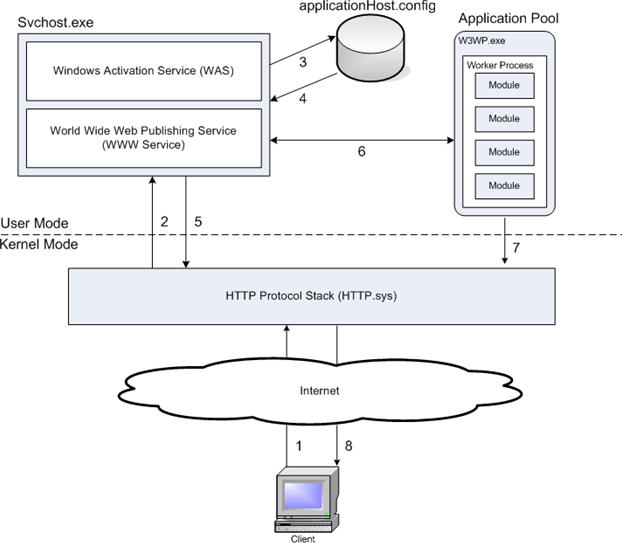
\includegraphics[width=0.65\textwidth]{requestProcessing.png}
			\vspace{-5mm}
			\attribution{MSDN}
		\end{center}
	\end{frame}

	\section{Архитектура ASP.NET MVC}

	\begin{frame}
		\frametitle{ASP.NET MVC, основные понятия}
		\begin{center}
			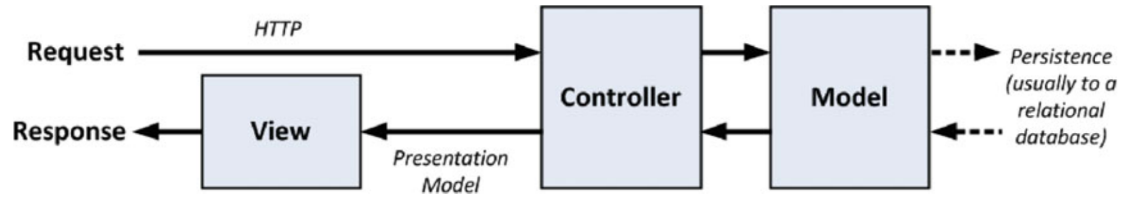
\includegraphics[width=0.7\textwidth]{mvc.png}
			\attribution{A. Freeman, Pro ASP.NET Core MVC}
		\end{center}

		\vspace{-5mm}

		\begin{itemize}
			\item \textbf{Модель} содержит или представляет данные, с которыми работает приложение
			\begin{itemize}
				\item \textbf{Domain model} содержит объекты предметной области вместе с бизнес-логикой, механизмами сериализации и т.д.
				\item \textbf{View Model} содержит классы, удобные для отображения во View, без бизнес-логики
			\end{itemize}
			\item \textbf{Представление} (View) отвечает за показ данных из модели пользователю
			\begin{itemize}
				\item Работает в браузере, но генерится на сервере
			\end{itemize}
			\item \textbf{Контроллер} отвечает за обработку входящих запросов, преобразование моделей и формирование данных для видов
		\end{itemize}
	\end{frame}

	\begin{frame}
		\frametitle{Типичная структура проекта ASP.NET}
		\begin{itemize}
			\item На самом деле, два шаблона проекта:
			\begin{itemize}
				\item Web Application --- Razor Pages, ``облегчённая версия''
				\item Web Application (Model-View-Controller) --- ``классическая'' версия
			\end{itemize}
			\item \textbf{wwwroot} --- статические ресурсы приложения (то, что можно включать в html-страницу), отправляются клиенту как есть
			\begin{itemize}
				\item favicon.ico --- картинка, показывающаяся в заголовке вкладки
			\end{itemize}
			\item \textbf{Pages} --- папка с Razor-разметкой, по которой будут генериться html-страницы
			\item \textbf{appsettings.json} --- конфигурация приложения
			\item \textbf{Program.cs} --- конфигурирует хост и запускает приложение
			\item \textbf{Startup.cs} --- конфигурирует сервисы и конвейер обработки запроса
		\end{itemize}
	\end{frame}

	\section{Razor}

	\begin{frame}
		\frametitle{Razor}
		\begin{itemize}
			\item Язык задания правил генерации
			\begin{itemize}
				\item Обычно используется для генерации веб-страниц, но может использоваться и независимо
			\end{itemize}
			\item Состоит из текста на целевом языке (в нашем случае html), кода на C\# и Razor-разметки, которая собирает всё это воедино
			\item Сервер исполняет Razor-код, используя данные \textit{модели} для генерации итоговой html-ки, которую и отправляет клиенту
		\end{itemize}
	\end{frame}

	\begin{frame}
		\frametitle{Синтаксис Razor}
		\begin{itemize}
			\item HTML-разметка пишется как есть
			\item Блоки кода заключаются в \mintinline{text}|@{ }|
			\item Один оператор можно писать без скобок: \mintinline{text}|The time is @DateTime.Now|
			\begin{itemize}
				\item Обратите внимание, Razor-код выполняется на сервере!
			\end{itemize}
			\item Выражения можно заключать в круглые скобки: \mintinline{text}|@(someValue * 10)|
			\item Всё, что выводится через \mintinline{text}|@|, кодируется вызовом HttpServerUtility.HtmlEncode
		\end{itemize}
	\end{frame}

	\begin{frame}[fragile]
		\frametitle{Пример}
		\begin{minted}{csharp}
@page

<h1>Cthulhu fhtagn!</h1>

@for (int i = 0; i < 300; ++i)
{
    <p>Cthulhu fhtagn!</p>
}
		\end{minted}
	\end{frame}

	\begin{frame}
		\frametitle{Синтаксис Razor (2)}
		\begin{itemize}
			\item Razor сам пытается угадать, где разметка, а где код
			\begin{itemize}
				\item Но у него не всегда получается
			\end{itemize}
			\item После \mintinline{text}|@| и до пробела (или до конца оператора) --- код
			\item После открывающего тэга --- разметка
			\item После \mintinline{text}|@:| --- HTML-разметка
			\item \mintinline{text}|@* ... *@| --- комментарии (серверные, не отправляются клиенту)
			\item \mintinline{text}|@@| --- \mintinline{text}|@| в HTML (escaping)
		\end{itemize}
	\end{frame}

	\begin{frame}
		\frametitle{Хелперы}
		\begin{itemize}
			\item Функции, которые генерируют HTML-код
			\item Есть много стандартных
			\begin{itemize}
				\item Html.BeginForm
				\item Html.TextBox
				\item Html.CheckBox
				\item ...
				\item Html.ActionLink
			\end{itemize}
			\item Ещё бывают TagHelper-ы:
			
			\mintinline{text}|@addTagHelper *, Microsoft.AspNetCore.Mvc.TagHelpers|
		\end{itemize}
	\end{frame}

	\section{Модели}

	\begin{frame}[fragile]
		\frametitle{Модели}
		\begin{itemize}
			\item Всё, что выше, не сильно полезнее статической HTML
			\item Реальное веб-приложение использует данные из модели
		\end{itemize}
		\begin{minted}{csharp}
@page
@using RazorPagesIntro.Pages
@model IndexModel2

<h2>Separate page model</h2>
<p>
    @Model.Message
</p>
		\end{minted}
	\end{frame}

	\begin{frame}[fragile]
		\frametitle{Code behind}
		\begin{small}
			\begin{minted}{csharp}
using Microsoft.AspNetCore.Mvc.RazorPages;
using System;

namespace RazorPagesIntro.Pages
{
    public class IndexModel2 : PageModel
    {
        public string Message { get; private set; } = "PageModel in C#";

        public void OnGet()
        {
            Message += $" Server time is { DateTime.Now }";
        }
    }
}
			\end{minted}
		\end{small}
		\attribution{MSDN}
	\end{frame}

	\section{Routing}

	\begin{frame}
		\frametitle{Routing}
		\framesubtitle{Или как ASP.NET находит по запросу страницу}
		\begin{itemize}
			\item Convention over configuration --- пока вы выполняете соглашения об именовании, по умолчанию всё происходит за вас
			\item Есть возможность конфигурировать роутинг вручную
			\item Соглашения:
			\begin{itemize}
				\item URL вида ``адрес сайта/'' или ``адрес сайта/Index'' отображаются в /Pages/Index.cshtml
				\item /Pages/Contact.cshtml --- URL вида ``адрес сайта/Contact''
				\item /Pages/Store/Contact.cshtml --- ``адрес сайта/Store/Contact''
				\item /Pages/Store/Index.cshtml --- ``адрес сайта/Store'' или ``адрес сайта/Store/Index''
			\end{itemize}
		\end{itemize}
	\end{frame}

	\begin{frame}
		\frametitle{Как всё вообще обрабатывается}
		\begin{center}
			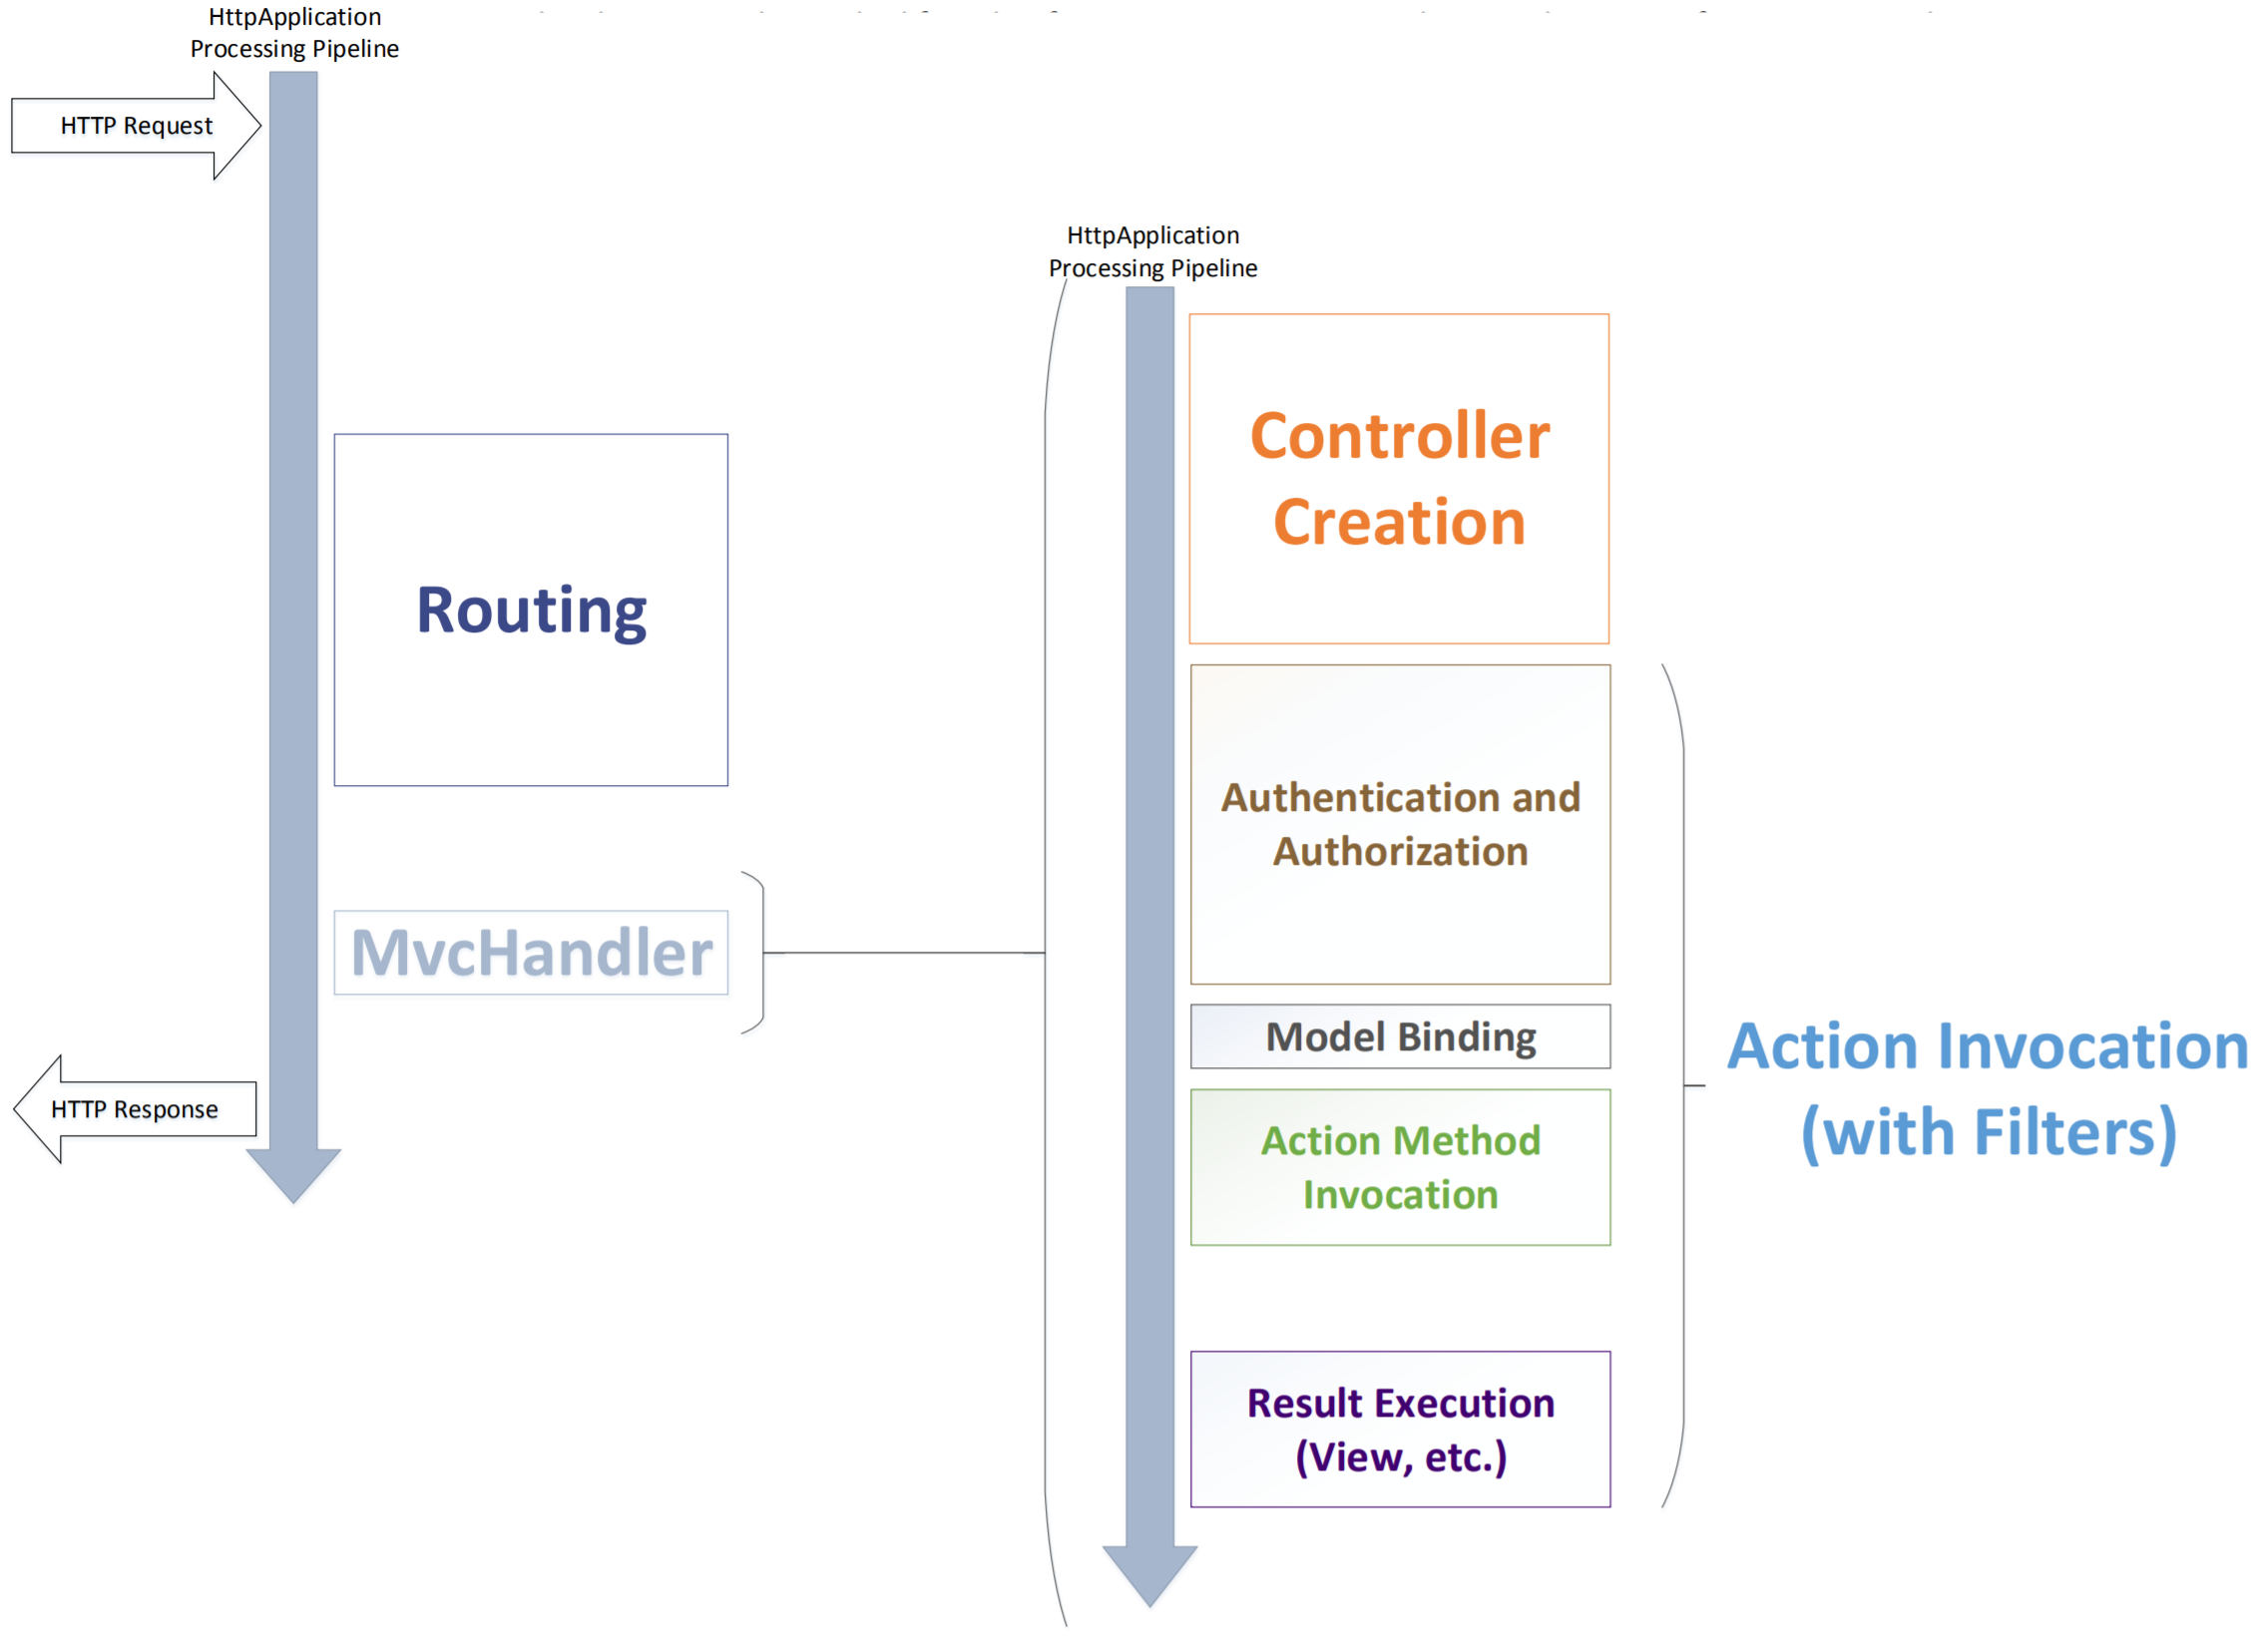
\includegraphics[width=0.85\textwidth]{requestLifecycle.png}
			\vspace{-5mm}
			\attribution{MSDN}
		\end{center}
	\end{frame}

	\section{Model binding}

	\begin{frame}[fragile]
		\frametitle{Model binding}
		\framesubtitle{Или как передать в Code Behind параметры}
		\begin{small}
			\begin{minted}{html}
@page
@model WebApplication1.Pages.IndexModel
@addTagHelper *, Microsoft.AspNetCore.Mvc.TagHelpers

<html>
<body>
    <p>
        Enter your name:
    </p>
    <form method="post">
        Name: <input type="text" name="name" />
        <input type="submit" />
    </form>
</body>
</html>
			\end{minted}
		\end{small}
		(GET тоже будет работать)
	\end{frame}

	\begin{frame}[fragile]
		\frametitle{Способ 1: в параметрах обработчика}
		\begin{small}
			\begin{minted}{csharp}
namespace WebApplication1.Pages
{
    public class IndexModel : PageModel
    {
        public void OnGet()
        {

        }

        public void OnPost(string name)
        {
            Console.WriteLine(name);
        }
    }
}
			\end{minted}
		\end{small}
	\end{frame}

	\begin{frame}[fragile]
		\frametitle{Способ 2: вручную}
		\begin{small}
			\begin{minted}{csharp}
public void OnPost()
{
    var name = Request.Form["name"];
    Console.WriteLine(name);
}
			\end{minted}
		\end{small}
	\end{frame}

	\begin{frame}[fragile]
		\frametitle{Способ 3: через свойства}
		\begin{small}
			\begin{minted}{csharp}
[BindProperty]
public string Name { get; set; }

public void OnPost()
{
    Console.WriteLine(Name);
}
			\end{minted}
		\end{small}
	\end{frame}

	\section{Большой пример}

	\begin{frame}
		\frametitle{Теперь попробуем написать что-нибудь ``настоящее''}
		\begin{itemize}
			\item Приложение для регистрации на конференцию
			\item Титульная страница конференции со ссылкой на форму регистрации
			\item Форма регистрации
			\begin{itemize}
				\item Как слушатель или как докладчик
			\end{itemize}
			\item Страница, на которой можно просмотреть всех зарегистрировавшихся
		\end{itemize}
	\end{frame}

	\begin{frame}[fragile]
		\frametitle{Моделирование предметной области}
		\begin{minted}{csharp}
public class Participant
{
    public int Id { get; set; }
    public string Name { get; set; }
    public string Email { get; set; }
    public bool? Speaker { get; set; }
}
		\end{minted}
	\end{frame}

	\begin{frame}[fragile]
		\frametitle{Титульная страница}
		\begin{minted}{html}
@page
@addTagHelper *, Microsoft.AspNetCore.Mvc.TagHelpers

<html>
<body>
    <h1>SEIM-2020</h1>
    <p>Coolest conference ever</p>
    <p>Please register:</p>
    <a asp-page="Register">Register</a>
</body>
</html>
		\end{minted}
	\end{frame}

	\begin{frame}[fragile]
		\frametitle{Страница регистрации}
		\begin{ssmall}
			\begin{minted}{html}
@page
@model WebApplication1.Pages.RegisterModel
@addTagHelper *, Microsoft.AspNetCore.Mvc.TagHelpers

<html>
<body>
    <form asp-action="Register" method="post">
        <p>
            <label asp-for="Participant.Name">Your name:</label>
            <input asp-for="Participant.Name" />
        </p>
        <p>
            <label asp-for="Participant.Email">Your email:</label>
            <input asp-for="Participant.Email" />
        </p>
        <p>
            <label>Are you a speaker?</label>
            <select asp-for="Participant.Speaker">
                <option value="">Choose an option</option>
                <option value="true">Yes</option>
                7
                <option value="false">No</option>
            </select>
        </p>
        <button type="submit">Register!</button>
    </form>
</body>
</html>
			\end{minted}
		\end{ssmall}
	\end{frame}

	\begin{frame}[fragile]
		\frametitle{Code behind}
		\begin{footnotesize}
			\begin{minted}{csharp}
public class RegisterModel : PageModel
{
    public void OnGet()
    {
    }

    [BindProperty]
    public Data.Participant Participant { get; set; }

    public IActionResult OnPost()
    {
        if (!ModelState.IsValid)
        {
            return Page();
        }

        return RedirectToPage($"/Thanks", new { name = Participant.Name });
    }
}
			\end{minted}
		\end{footnotesize}
	\end{frame}

	\begin{frame}[fragile]
		\frametitle{Страница благодарности}
		\begin{small}
			\begin{minted}{html}
@page "{name}"

<html>
<body>
    <h1>Thanks for registration, @RouteData.Values["name"]!</h1>
</body>
</html>
			\end{minted}
		\end{small}
	\end{frame}

	\begin{frame}[fragile]
		\frametitle{Добавим немного СУБД}
		\framesubtitle{Класс Data.AppDbContext}
		\begin{small}
			\begin{minted}{csharp}
public class AppDbContext: DbContext
{
    public AppDbContext(DbContextOptions options)
        : base(options)
    {
    }

    public DbSet<Participant> Participants { get; set; }
}
			\end{minted}
		\end{small}
	\end{frame}

	\begin{frame}[fragile]
		\frametitle{Но где же Connection String?}
		\begin{itemize}
			\item Dependency Injection --- архитектурный паттерн, отделяющий создание и конфигурирование объектов от их логики
			\item За создание и конфигурирование/переконфигурирование отвечает DI-контейнер, обычно отдельная подсистема
			\item Мы лишь описываем ограничения на то, что должно получиться
			\item Конкретно в нашем случае:
			\begin{itemize} 
				\item Подключаем пакет Microsoft.EntityFrameworkCore.Sqlite
				\item Пишем в Startup.ConfigureServices:
				\begin{minted}{csharp}
services.AddDbContext<Data.AppDbContext>(
    options => options.UseSqlite(@"Data source=Test.db;"));
				\end{minted}
			\end{itemize}
			\item DI-контейнер создаёт и регистрирует контекст, передавая ему в конструктор опции
		\end{itemize}
	\end{frame}

	\begin{frame}
		\frametitle{Инициализация базы данных}
		\begin{itemize}
			\item Идём ВНЕЗАПНО в Tools -> Nuget Package Manager -> Package Manager Console
			\item Набираем в консоли Add-Migration Initial
			\begin{itemize}
				\item Создаётся \textit{миграция}, которая создаст базу
			\end{itemize}
			\item Набираем в консоли Update-Database
			\begin{itemize}
				\item Миграция применяется, в папке с проектом создаётся Test.db
			\end{itemize}
		\end{itemize}
	\end{frame}

	\begin{frame}[fragile]
		\frametitle{Пришла пора воспользоваться СУБД}
		\begin{ssmall}
			\begin{minted}{csharp}
public class RegisterModel : PageModel
{
    private readonly AppDbContext db;

    public RegisterModel(AppDbContext db)
    {
        this.db = db;
    }

    [BindProperty]
    public Participant Participant { get; set; }

    public async Task<IActionResult> OnPostAsync()
    {
        if (!ModelState.IsValid)
        {
            return Page();
        }

        db.Participants.Add(Participant);
        await db.SaveChangesAsync();

        return RedirectToPage($"/Thanks", new { name = Participant.Name });
    }
}
			\end{minted}
		\end{ssmall}
	\end{frame}

	\begin{frame}[fragile]
		\frametitle{Ну и последняя страница, просмотр участников}
		\framesubtitle{Code Behind}
		\begin{scriptsize}
			\begin{minted}{csharp}
public class ViewModel : PageModel
{
    private readonly AppDbContext db;

    public ViewModel(AppDbContext db)
    {
        this.db = db;
    }

    public IList<Participant> Participants { get; private set; }

    public async Task OnGetAsync()
    {
        Participants = await db.Participants.AsNoTracking().ToListAsync();
    }
}
			\end{minted}
		\end{scriptsize}
	\end{frame}

	\begin{frame}[fragile]
		\frametitle{.cshtml}
		\begin{ssmall}
			\begin{minted}{html}
@page
@model WebApplication1.Pages.ViewModel

<html>
<body>
    <table class="table">
        <thead>
            <tr>
                <th>ID</th>
                <th>Name</th>
                <th>Email</th>
                <th>Is Speaker</th>
            </tr>
        </thead>
        <tbody>
            @foreach (var participant in Model.Participants)
            {
            <tr>
                <td>@participant.Id</td>
                <td>@participant.Name</td>
                <td>@participant.Email</td>
                <td>@(participant.Speaker == true ? "Yes" : "No")</td>
            </tr>
            }
        </tbody>
    </table>
</body>
</html>
			\end{minted}
		\end{ssmall}
	\end{frame}

	\begin{frame}[fragile]
		\frametitle{Но так даже в 90-е не верстали!}
		\framesubtitle{Добавим Bootstrap}
		\begin{tiny}
			\begin{minted}{html}
@page
@model WebApplication1.Pages.ViewModel

<html>
<head>
    <link rel="stylesheet" href="/lib/bootstrap/dist/css/bootstrap.css" />
</head>
<body>
    <table class="table table-striped table-bordered">
        <thead>
            <tr>
                <th scope="col">ID</th>
                <th scope="col">Name</th>
                <th scope="col">Email</th>
                <th scope="col">Is Speaker</th>
            </tr>
        </thead>
        <tbody>
            @foreach (var participant in Model.Participants)
            {
            <tr>
                <td>@participant.Id</td>
                <td>@participant.Name</td>
                <td>@participant.Email</td>
                <td>@(participant.Speaker == true ? "Yes" : "No")</td>
            </tr>
            }
        </tbody>
    </table>
</body>
</html>
			\end{minted}
		\end{tiny}
	\end{frame}

\end{document}
